\chap{LED Animations}


\section{Exercise and Report}
\subsection{Exercise 1}
% From the simulation on Proteus, one more LED is connected to pin \textbf{PA6} of the STM32 (negative pin of the LED is connected to PA6). The component suggested in this exercise is \textbf{LED-YELLOW}, which can be found from the device list.\\



% In this exercise, the status of two LEDs are switched every 2 seconds, as demonstrated in the figure bellow.

\begin{figure}[!htp]
    \centering
    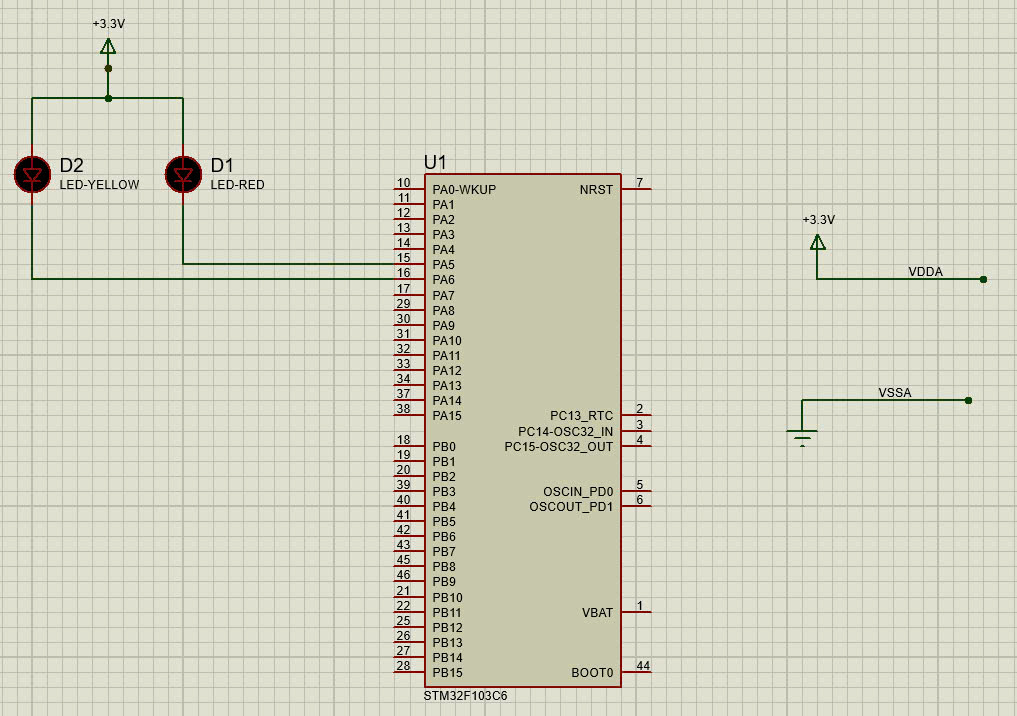
\includegraphics[width=5in]{source/picture/bai_1/pic1.jpg}
    \caption{\textit{Schematic}}
    \label{bai1_pic1}
\end{figure}

% \textbf{Report 1: }Depict the schematic from Proteus simulation in this report. The caption of the figure is a downloadable link to the Proteus project file (e.g. a github link).\\

% \textbf{Report 2: } Present the source code in the infinite loop while of your project. If a user-defined functions is used, it is required to present in this part. A brief description can be added for this function (e.g. using comments). A template to present your source code is presented bellow.

\begin{lstlisting}[caption= main.c]
while (1){
HAL_GPIO_WritePin(LED_RED_GPIO_Port, LED_RED_Pin, RESET);   
HAL_GPIO_WritePin(LED_YELLOW_GPIO_Port,LED_YELLOW_Pin,SET);
HAL_Delay(2000);
HAL_GPIO_WritePin(LED_RED_GPIO_Port, LED_RED_Pin, SET);
HAL_GPIO_WritePin(LED_YELLOW_GPIO_Port,LED_YELLOW_Pin,RESET); 
HAL_Delay(2000);
}
\end{lstlisting}
\newpage
\subsection{Exercise 2}
\begin{figure}[!htp]
    \centering
    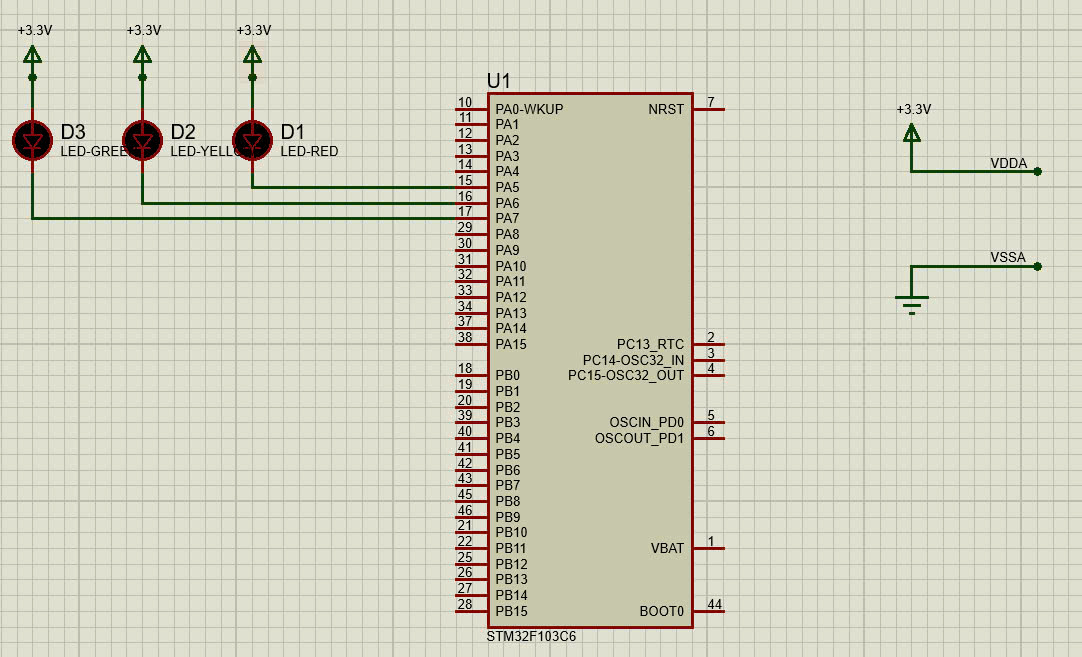
\includegraphics[width=5in]{source/picture/bai_1/pic2.jpg}
    \caption{\textit{Schematic}}
    \label{bai1_pic1}
\end{figure}

\begin{lstlisting}[caption= main.c]
while (1){
	  	  HAL_GPIO_WritePin(LED_RED_GPIO_Port, LED_RED_Pin, RESET);  
	  	  HAL_GPIO_WritePin(LED_YELLOW_GPIO_Port, LED_YELLOW_Pin, SET);
	  	  HAL_GPIO_WritePin(LED_GREEN_GPIO_Port, LED_GREEN_Pin, SET);
	  	  HAL_Delay(5000);
	  	  HAL_GPIO_WritePin(LED_GREEN_GPIO_Port, LED_GREEN_Pin, RESET);
	  	  HAL_GPIO_WritePin(LED_RED_GPIO_Port, LED_RED_Pin, SET);
	  	  HAL_GPIO_WritePin(LED_YELLOW_GPIO_Port, LED_YELLOW_Pin, SET); 
	  	  HAL_Delay(3000);
	  	  HAL_GPIO_WritePin(LED_YELLOW_GPIO_Port, LED_YELLOW_Pin, RESET); 
	  	  HAL_GPIO_WritePin(LED_GREEN_GPIO_Port, LED_GREEN_Pin, SET);
	  	  HAL_GPIO_WritePin(LED_RED_GPIO_Port, LED_RED_Pin, SET);
	  	  HAL_Delay(2000);
}
\end{lstlisting}
\newpage
\subsection{Exercise 3}

\begin{figure}[!htp]
    \centering
    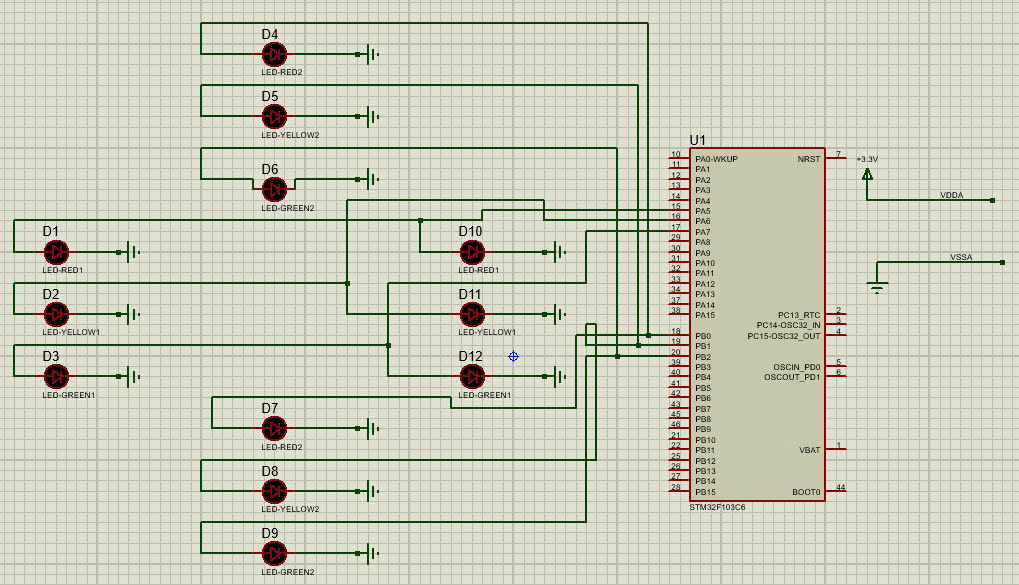
\includegraphics[width=5in]{source/picture/bai_1/pic3.jpg}
    \caption{\textit{Schematic}}
    \label{bai1_pic2}
\end{figure}
\begin{lstlisting}[caption= Ex3.c]
void settrafficlight1(GPIO_TypeDef* LED_GIPO_Port, uint16_t LED_Pin,GPIO_TypeDef* LED_1GIPO_Port, uint16_t LED_1Pin,GPIO_TypeDef* LED_2GIPO_Port, uint16_t LED_2Pin)
  {
	  HAL_GPIO_WritePin(LED_GIPO_Port, LED_Pin, SET);
	  HAL_GPIO_WritePin(LED_1GIPO_Port, LED_1Pin, RESET);
	  HAL_GPIO_WritePin(LED_2GIPO_Port, LED_2Pin, RESET);
  }
\end{lstlisting}

\begin{lstlisting}[caption= main.c]
while (1){
settrafficlight1(LED_RED1_GPIO_Port,LED_RED1_Pin,LED_YELLOW1_GPIO_Port, LED_YELLOW1_Pin, LED_GREEN1_GPIO_Port, LED_GREEN1_Pin);
settrafficlight1(LED_GREEN2_GPIO_Port, LED_GREEN2_Pin, LED_RED2_GPIO_Port, LED_RED2_Pin, LED_YELLOW2_GPIO_Port, LED_YELLOW2_Pin) ;
HAL_Delay(3000);
settrafficlight1(LED_YELLOW2_GPIO_Port, LED_YELLOW2_Pin, LED_GREEN2_GPIO_Port, LED_GREEN2_Pin, LED_RED2_GPIO_Port, LED_RED2_Pin);
HAL_Delay(2000);
settrafficlight1(LED_RED2_GPIO_Port, LED_RED2_Pin, LED_YELLOW2_GPIO_Port, LED_YELLOW2_Pin, LED_GREEN2_GPIO_Port, LED_GREEN2_Pin);
settrafficlight1(LED_GREEN1_GPIO_Port, LED_GREEN1_Pin, LED_RED1_GPIO_Port, LED_RED1_Pin, LED_YELLOW1_GPIO_Port, LED_YELLOW1_Pin);
HAL_Delay(3000);
settrafficlight1(LED_YELLOW1_GPIO_Port, LED_YELLOW1_Pin, LED_GREEN1_GPIO_Port, LED_GREEN1_Pin, LED_RED1_GPIO_Port, LED_RED1_Pin);
HAL_Delay(2000);
}
\end{lstlisting}

\subsection{Exercise 4}


\begin{figure}[!htp]
    \centering
    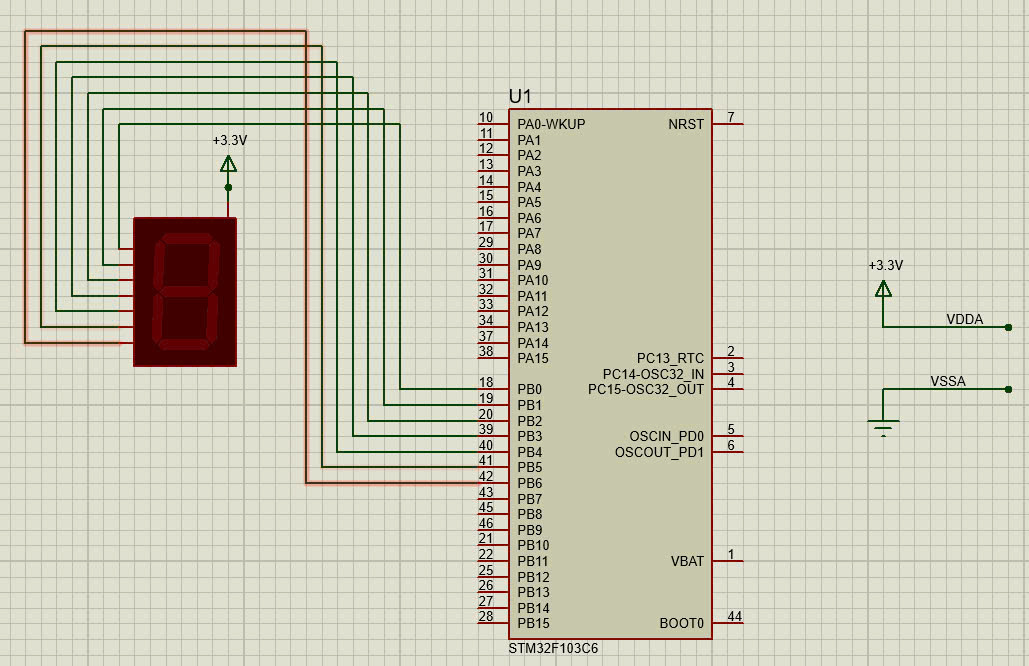
\includegraphics[width=5in]{source/picture/bai_1/pic4.jpg}
    \caption{\textit{Schematic}}
    \label{bai1_pic3}
\end{figure}
\begin{lstlisting}[caption=Ex4.c]
void display7SEG(int num) {
      const uint8_t segmentMap[10] = {
          0b11111100,
          0b01100000,
          0b11011010,
          0b11110010,
          0b01100110,
          0b10110110,
          0b10111110,
          0b11100000,
          0b11111110,
          0b11110110
      };
  HAL_GPIO_WritePin(a_GPIO_Port, a_Pin, (segmentMap[num] & 0b10000000) ? GPIO_PIN_RESET : GPIO_PIN_SET);
  HAL_GPIO_WritePin(b_GPIO_Port, b_Pin, (segmentMap[num] & 0b01000000) ? GPIO_PIN_RESET : GPIO_PIN_SET);
  HAL_GPIO_WritePin(c_GPIO_Port, c_Pin, (segmentMap[num] & 0b00100000) ? GPIO_PIN_RESET : GPIO_PIN_SET);
  HAL_GPIO_WritePin(d_GPIO_Port, d_Pin, (segmentMap[num] & 0b00010000) ? GPIO_PIN_RESET : GPIO_PIN_SET);
  HAL_GPIO_WritePin(e_GPIO_Port, e_Pin, (segmentMap[num] & 0b00001000) ? GPIO_PIN_RESET : GPIO_PIN_SET);
  HAL_GPIO_WritePin(f_GPIO_Port, f_Pin, (segmentMap[num] & 0b00000100) ? GPIO_PIN_RESET : GPIO_PIN_SET);
  HAL_GPIO_WritePin(g_GPIO_Port, g_Pin, (segmentMap[num] & 0b00000010) ? GPIO_PIN_RESET : GPIO_PIN_SET);
  }
\end{lstlisting}

\begin{lstlisting}[caption=main.c]
int counter = 0;
while (1){
    if(counter >= 10) counter = 0;    
    display7SEG(counter++);
    HAL_Delay(1000);

}
\end{lstlisting}



\subsection{Exercise 5}
\begin{figure}[!htp]
    \centering
    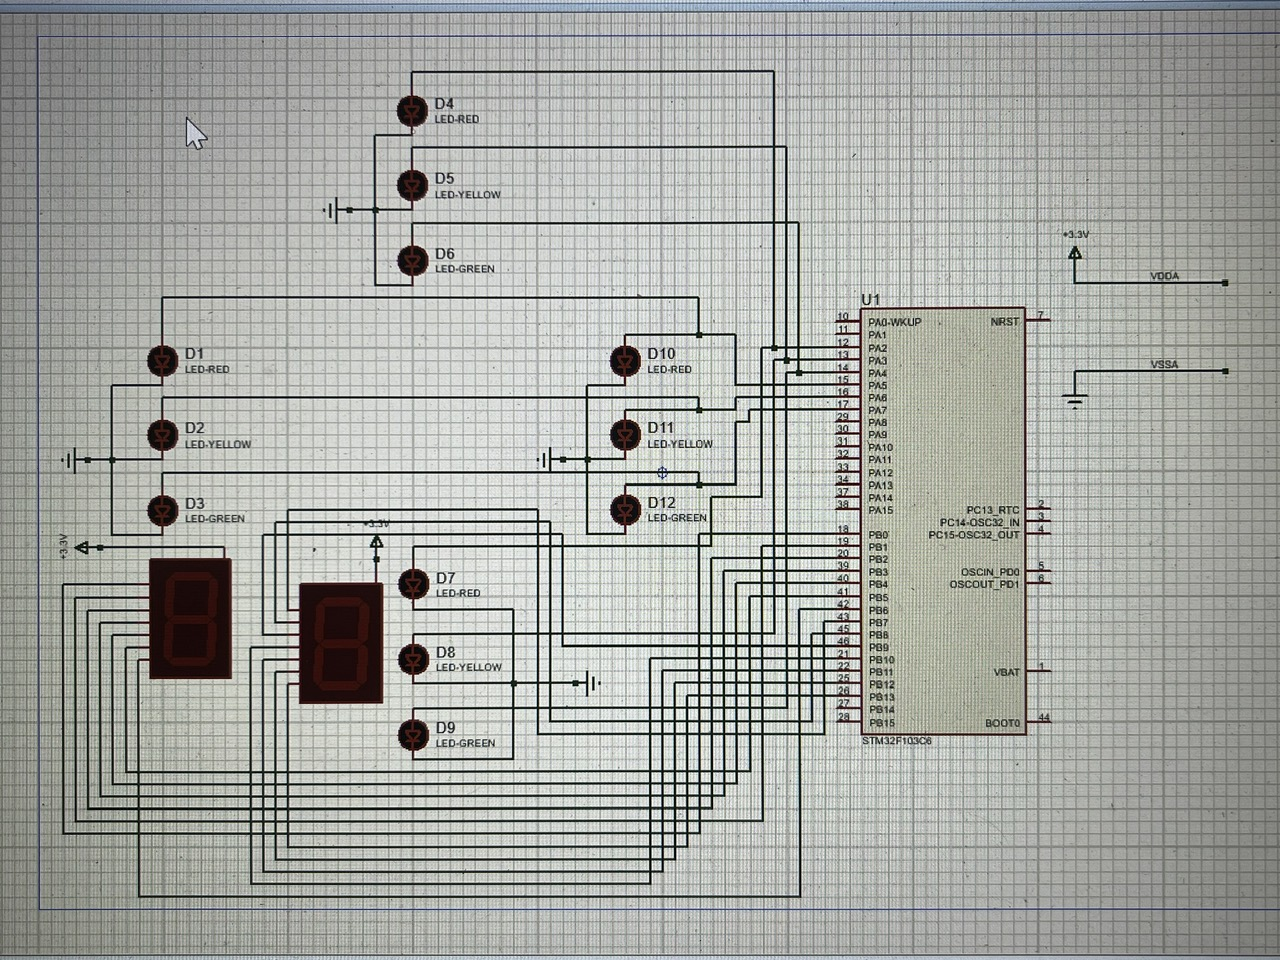
\includegraphics[width=5in]{source/picture/bai_1/pic5.jpg}
    \caption{\textit{Schematic}}
    \label{bai1_pic3}
\end{figure}
\begin{lstlisting}[caption=Ex5.c]
int counterred=6;
  int counteryellow=2;
  int countergreen=3;
GPIO_TypeDef* segmentPorts[2][NUM_SEGMENTS] = {
      {a1_GPIO_Port, b1_GPIO_Port, c1_GPIO_Port, d1_GPIO_Port, e1_GPIO_Port, f1_GPIO_Port, g1_GPIO_Port},  
      {a2_GPIO_Port, b2_GPIO_Port, c2_GPIO_Port, d2_GPIO_Port, e2_GPIO_Port, f2_GPIO_Port, g2_GPIO_Port}   
  };
  uint16_t segmentPins[2][NUM_SEGMENTS] = {
      {a1_Pin, b1_Pin, c1_Pin, d1_Pin, e1_Pin, f1_Pin, g1_Pin},  
      {a2_Pin, b2_Pin, c2_Pin, d2_Pin, e2_Pin, f2_Pin, g2_Pin}   
  };
  const uint8_t segmentMap[10] = {
        0b11111100,  
        0b01100000,  
        0b11011010,  
        0b11110010,  
        0b01100110,  
        0b10110110,  
        0b10111110, 
        0b11100000, 
        0b11111110,  
        0b11110110  
    };
  void settrafficlight1(GPIO_TypeDef* LED_GIPO_Port, uint16_t LED_Pin,GPIO_TypeDef* LED_1GIPO_Port, uint16_t LED_1Pin,GPIO_TypeDef* LED_2GIPO_Port, uint16_t LED_2Pin){
    	  HAL_GPIO_WritePin(LED_GIPO_Port, LED_Pin, SET);
    	  HAL_GPIO_WritePin(LED_1GIPO_Port, LED_1Pin, RESET);
    	  HAL_GPIO_WritePin(LED_2GIPO_Port, LED_2Pin, RESET);
      }
  void display7SEG(int ledNum, int num) {
        for (int i = 0; i < NUM_SEGMENTS; i++) {
            HAL_GPIO_WritePin(segmentPorts[ledNum][i], segmentPins[ledNum][i],
                              (segmentMap[num] & (0b10000000 >> i)) ? RESET : SET);
        }
    }
  void process(){
  	  settrafficlight1(LED_RED1_GPIO_Port, LED_RED1_Pin, LED_YELLOW1_GPIO_Port, LED_YELLOW1_Pin, LED_GREEN1_GPIO_Port, LED_GREEN1_Pin);
  	  settrafficlight1(LED_GREEN2_GPIO_Port, LED_GREEN2_Pin, LED_RED2_GPIO_Port, LED_RED2_Pin, LED_YELLOW2_GPIO_Port, LED_YELLOW2_Pin) ;
        for(int i=5;i>=2;i--){
      	  display7SEG(0, counterred--);
      	  display7SEG(1, countergreen--);
      	  HAL_Delay(1000);
        }
        settrafficlight1(LED_YELLOW2_GPIO_Port, LED_YELLOW2_Pin, LED_GREEN2_GPIO_Port, LED_GREEN2_Pin, LED_RED2_GPIO_Port, LED_RED2_Pin);
  	  for(int i=2;i>=0;i--){
  		  display7SEG(0, counterred--);
  		  display7SEG(1, counteryellow--);
  		  HAL_Delay(1000);
  		  if(i<=0){
  			  counterred=6;
  			  counteryellow=2;
  			  countergreen=3;
  		  }
  	  }
  	  settrafficlight1(LED_RED2_GPIO_Port, LED_RED2_Pin, LED_YELLOW2_GPIO_Port, LED_YELLOW2_Pin, LED_GREEN2_GPIO_Port, LED_GREEN2_Pin);
  	  settrafficlight1(LED_GREEN1_GPIO_Port, LED_GREEN1_Pin, LED_RED1_GPIO_Port, LED_RED1_Pin, LED_YELLOW1_GPIO_Port, LED_YELLOW1_Pin);
  	  for(int i=5;i>=2;i--){
  	      	  display7SEG(1, counterred--);
  	      	  display7SEG(0, countergreen--);
  	      	HAL_Delay(1000);
  	  }
  	  settrafficlight1(LED_YELLOW1_GPIO_Port, LED_YELLOW1_Pin, LED_GREEN1_GPIO_Port, LED_GREEN1_Pin, LED_RED1_GPIO_Port, LED_RED1_Pin);
  	  for(int i=2;i>=0;i--){
  		  	  display7SEG(1, counterred--);
  	  		  display7SEG(0, counteryellow--);
  	  		HAL_Delay(1000);
  	  		if(i<=0){
  	  			counterred=6;
  	  			counteryellow=2;
  	  			countergreen=3;
  	  		}
  	  }
    }
\end{lstlisting}
\begin{lstlisting}[caption=main.c]
while (1){
	    process();
}
\end{lstlisting}
\newpage
\subsection{Exercise 6}


\begin{figure}[!htp]
    \centering
    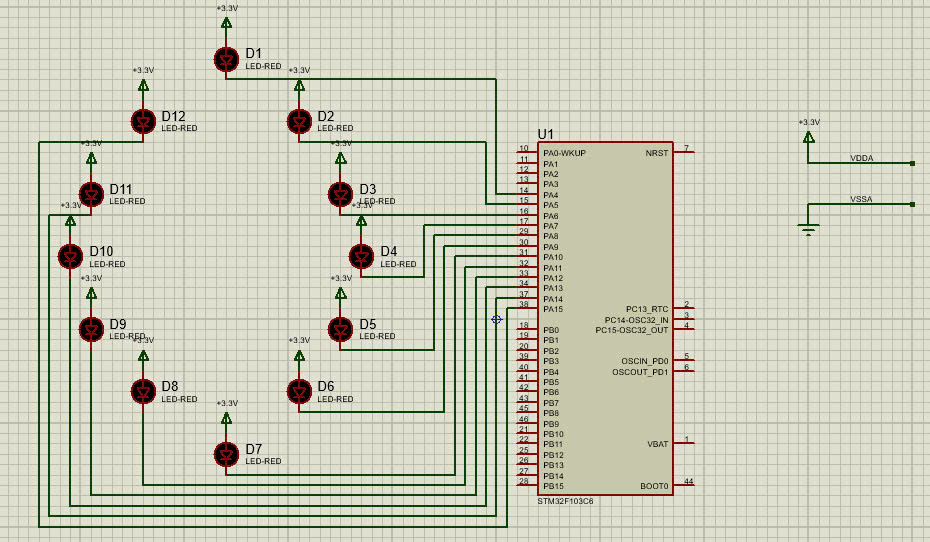
\includegraphics[width=5in]{source/picture/bai_1/pic6.jpg}
    \caption{\textit{Schematic}}
    \label{bai1_pic3}
\end{figure}
\begin{lstlisting}[caption=Ex6.c]
int counter=0;
GPIO_TypeDef* segmentPorts[12] = {
      LED0_GPIO_Port, LED1_GPIO_Port,LED2_GPIO_Port,LED3_GPIO_Port,LED4_GPIO_Port,LED5_GPIO_Port,
	  LED6_GPIO_Port,LED7_GPIO_Port,LED8_GPIO_Port,LED9_GPIO_Port,LED10_GPIO_Port,LED11_GPIO_Port};
uint16_t segmentPins[12]={
    	LED0_Pin,LED1_Pin,LED2_Pin,LED3_Pin,LED4_Pin,LED5_Pin,LED6_Pin,LED7_Pin
    	                          ,LED8_Pin,LED9_Pin,LED10_Pin,LED11_Pin};
void TurnOnEveryClock(int num) {
          for (int i = 0; i < 12; i++) {
        	  if(i==num)HAL_GPIO_WritePin(segmentPorts[num], segmentPins[num], RESET);
        	  else HAL_GPIO_WritePin(segmentPorts[i], segmentPins[i], SET);
          }
      }
\end{lstlisting}
\begin{lstlisting}[caption=main.c]
while (1){
	  if(counter>=12) counter=0;
	  TurnOnEveryClock(counter++);
	  HAL_Delay(1000);
   }
\end{lstlisting}

\subsection{Exercise 7}

\begin{lstlisting}[caption=main.c]
void clearAllClock(){
    HAL_GPIO_WritePin(GPIOA, LED_PINS, SET);
}
\end{lstlisting}

\subsection{Exercise 8}
\begin{lstlisting}[caption=Ex8.c]
GPIO_TypeDef* segmentPorts[12] = {LED0_GPIO_Port,LED1_GPIO_Port,LED2_GPIO_Port,LED3_GPIO_Port,LED4_GPIO_Port,
LED5_GPIO_Port,LED6_GPIO_Port,LED7_GPIO_Port,LED8_GPIO_Port,LED9_GPIO_Port,LED10_GPIO_Port,LED11_GPIO_Port};
uint16_t segmentPins[12]={LED0_Pin,LED1_Pin,LED2_Pin,LED3_Pin,LED4_Pin,LED5_Pin,LED6_Pin,LED7_Pin
      	   ,LED8_Pin,LED9_Pin,LED10_Pin,LED11_Pin};
void clearNumberOnClock(int num) {
   HAL_GPIO_WritePin(segmentPorts[num], segmentPins[num], RESET);
 }

\end{lstlisting}


\subsection{Exercise 9}
\begin{lstlisting}[caption=Ex9.c]
GPIO_TypeDef* segmentPorts[12] = {LED0_GPIO_Port,LED1_GPIO_Port,LED2_GPIO_Port,LED3_GPIO_Port,LED4_GPIO_Port,
LED5_GPIO_Port,LED6_GPIO_Port,LED7_GPIO_Port,LED8_GPIO_Port,LED9_GPIO_Port,LED10_GPIO_Port,LED11_GPIO_Port};
uint16_t segmentPins[12]={LED0_Pin,LED1_Pin,LED2_Pin,LED3_Pin,LED4_Pin,LED5_Pin,LED6_Pin,LED7_Pin
      	   ,LED8_Pin,LED9_Pin,LED10_Pin,LED11_Pin};
void clearNumberOnClock(int num) {
   HAL_GPIO_WritePin(segmentPorts[num], segmentPins[num], SET);
 }

\end{lstlisting}

\subsection{Exercise 10}
\begin{lstlisting}[caption=Ex10.c]
int second=0;
int minute=0;
int hour=0;
GPIO_TypeDef* segmentPorts[12] = {LED0_GPIO_Port, LED1_GPIO_Port,LED2_GPIO_Port,LED3_GPIO_Port,LED4_GPIO_Port,
LED5_GPIO_Port,LED6_GPIO_Port,LED7_GPIO_Port,LED8_GPIO_Port,LED9_GPIO_Port,LED10_GPIO_Port,LED11_GPIO_Port};  // LED 1
uint16_t segmentPins[12]={LED0_Pin,LED1_Pin,LED2_Pin,LED3_Pin
  ,LED4_Pin,LED5_Pin,LED6_Pin,LED7_Pin,LED8_Pin,LED9_Pin,LED10_Pin,LED11_Pin};
void setClock(int num){
        	HAL_GPIO_WritePin(segmentPorts[num], segmentPins[num], RESET);
        }
void clearClock(int num){
        	HAL_GPIO_WritePin(segmentPorts[num], segmentPins[num], SET);
        }
void setClockBegin(int hour,int minute,int second){
        	HAL_GPIO_WritePin(segmentPorts[hour], segmentPins[hour], RESET);
        if(minute%5==0)	HAL_GPIO_WritePin(segmentPorts[minute/5], segmentPins[minute/5], RESET);
        if(second%5==0)	HAL_GPIO_WritePin(segmentPorts[second/5], segmentPins[second/5], RESET);
        HAL_Delay(2000);
        }

\end{lstlisting}
\begin{lstlisting}[caption=main.c]
setClockBegin(hour,minute,second);
  while (1)
  {
	  second++;
	  	      if (second >= 60) {
	  	          second = 0;
	  	          minute++;
	  	          setClock((minute / 5+12)%12);
        if(((minute / 5+11)%12)!=hour) clearClock(((minute / 5+11)%12));
	  	          if (minute >= 60) {
	  	              minute = 0;
	  	              hour++;
	  	              setClock((hour+12)%12);
	  	              if((hour+11)%12!=0) clearClock((hour+11)%12);
	  	              if (hour >= 12) {
	  	                  hour = 0;
	  	              }
	  	          }
	  	      }
	  	      setClock((second / 5+12)%12);
	  if(((second / 5+11)%12)!=hour&&((second / 5+11)%12)!=(minute/5+12)%12) clearClock(((second / 5+11)%12));
	  	      HAL_Delay(100);
        }
\end{lstlisting}